% первая часть

\section{Обзор существующей методики проведения процедуры КГО стендовым методом}

\subsection{Основные положения}

В данной работе рассматривается метод КГО в пеналах СОДС~\cite{RD}, который является одним из наиболее надёжных способов определения негерметичных ТВС. СОДС входит в состав обязательного оборудования всех действующих и проектируемых АЭС с реактором ВВЭР.

Метод основан на измерении утечки ПД из-под оболочек твэлов путем гамма-спектрометрического анализа изотопного состава проб воды, отбираемых из контура циркуляции СОДС, по активности реперных радионуклидов $^{131}$I, $^{134}$Cs, $^{136}$Cs, $^{137}$Cs и $^{133}$Xe. Инициирование выхода радионуклидов в воду стенда КГО осуществляется посредством изменения давления циркулирующей по контуру стенда воды в процессе выдержки ТВС в этой воде -- настаивании.

\subsection{Процедура проведения КГО стендовым методом}
1. Процедура проведения КГО начинается проведения испытаний для каждой ТВС в пеналах СОДС с последующим отбором проб воды. 

Проверка ТВС проводится при циркуляции воды по контуру стенда КГО без ее замены и состоит из двух циклов:
\begin{itemize}
\item Настаивание ТВС при изыбыточном (верхнем) давлении в контуре от 4,5 * 10$^{5}$ Па до 6,0 * 10$^{5}$ Па продолжительностью 5 минут.

\item Настаивание ТВС при избыточном (нижнем) давлении в контуре от 1,0 * 10$^{5}$ Па до 1,5 * 10$^{5}$ Па до полного перемешивания (не менее 15 минут).
\end{itemize}

С целью соблюдения одинаковых условий испытаний требуется, чтобы значения верхнего и нижнего избыточного давления были одинаковыми при проверке всех ТВС. 

2. После завершения настаивания ТВС производится отбор пробы воды из контура стенда КГО.

3. В каждой $j$-ой пробе воды, взятой из стенда КГО при испытании $j$-ой ТВС, на спектрометрической установке измеряются значения удельной активности и приводятся на момент останова реактора:
\begin{itemize}
\item $A_{j,кго}^{i}$ --- реперных $i$-х радионуклидов продуктов деления ($^{131}$I, $^{134}$Cs, $^{136}$Cs, $^{137}$Cs и $^{133}$Xe)

\item $A_{j,кго}^{i'}$ --- радионуклида продуктов коррозии(ПК) ($^{54}$Mn или $^{58}$Co, $^{60}$Co, $^{51}$Cr, $^{59}$Fe).
\end{itemize}

4. Для учета фоновой активности радионуклидов йода, цезия и
продуктов коррозии периодически производится измерение их активности
в воде, подаваемой в стенд КГО (с каждой вновь приготовленной порцией
раствора борной кислоты на СВО), и в бассейне выдержки (один раз в
сутки).

5. Проверка фоновой составляющей за счет загрязнения стенда
радиоактивными продуктами (холостая проба) производится перед началом
работ по КГО, а также периодически (не реже одного раза в сутки). Для этого
без загрузки ТВС в пенал проводятся все операции по промывке контура и
настаиванию с отбором и анализом пробы.

6. Итогом проведения спектрометрического анализа проб воды является
таблица значений, в которых для каждой $j$-ой ТВС приводятся в соответствие
значения активности $A_{j,кго}^{i}$ каждого из регистрируемых реперных радионуклидов
и $A_{j,кго}^{i'}$ продуктов коррозии. Статистический анализ результатов
измерения проводится для ТВС, в пробах которых значимо регистрировались
ПД. Результаты измерений ТВС, при проверке которых реперные ПД не
регистрировались, из статистического расчета исключаются.

\subsection{Обработка результатов}
1. Анализ герметичности ТВС, согласно~\cite{RD}, основан на выборочном поиске выбросов методом "трёх сигм".

2. Основными реперными радионуклидами, по которым устанавливается наличие(отсутствие) негерметичных твэлов в ТВС являются $^{131}$I, $^{134}$Cs, $^{137}$Cs. Наличие в контролируемой пробе $^{136}$Cs и(или) $^{133}$Xe, значимо превышающих их содержание в холостых пробах, является однозначным основанием для включение ТВС в список подозрительных, требующих как минимум дополнительной проверки.

3. Полученные значения представляются в графическом виде в такой
хронологической последовательности, в какой ТВС проверялись в стенде
КГО. Примеры графического представления результатов КГО приведены на
рисунках~\ref{fig:ris1} и~\ref{fig:ris2}. На основании визуального анализа этих данных на графике
может быть сделано заключение, относятся ли они к одному статистическому
распределению. Таким способом проводится оценка соблюдения одинаковых
условий проверки всех ТВС.\label{distribution} Если условия менялись с течением времени (на
практике так происходит почти всегда), то производится разделение исходных данных на выборки, которые относятся к одному статистическому распределению.

\begin{figure}[H]
	\centering
	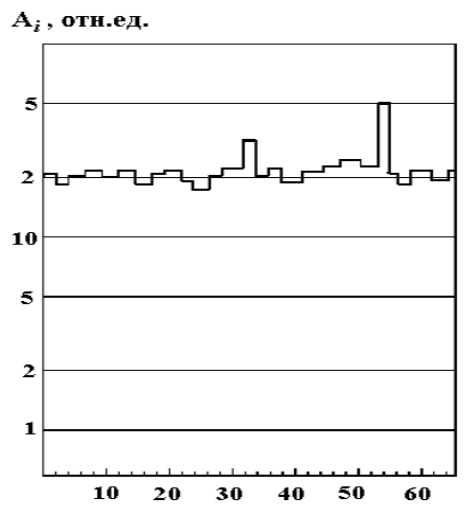
\includegraphics[width=0.5\linewidth]{pics/ris1} % изображения хранятся в подкаталоге pics
	\caption{Графическое хронологическое представление данных, принадлежащих к одному распределению.~\cite{RD}}
	\label{fig:ris1} % эта метка позволяет ссылаться на рисунок в тексте
\end{figure}

\begin{figure}[H]
	\centering
	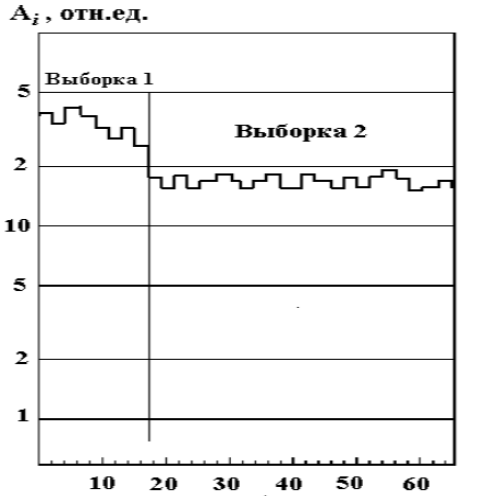
\includegraphics[width=0.5\linewidth]{pics/ris2} % изображения хранятся в подкаталоге pics
	\caption{Графическое хронологическое представление данных, принадлежащих к различным распределениям.~\cite{RD}}
	\label{fig:ris2} % эта метка позволяет ссылаться на рисунок в тексте
\end{figure}

4. Для каждой полученной совокупности данных, относящихся к одному
и тому же статистическому распределению, вычисляются $\overline{A}_{кго}^{i}$ --- среднеарифметические значения удельной активности радионуклидов $^{131}$I (и $^{134}$Cs, $^{136}$Cs, $^{137}$Cs, $^{133}$Xe) и $\overline{A}_{кго}^{i'}$ --- среднеарифметическое значение удельной активности $^{54}$Mn (или $^{58}$Co, $^{60}$Co, $^{51}$Cr, $^{59}$Fe), по формулам~\ref{eq:Mean} и~\ref{eq:corosionMean}:

\begin{equation} \label{eq:Mean}
	\overline{A}_{кго}^{i} = \frac{1}{N}\sum_{j=1}^{N}A_{j,кго}^{i}.
\end{equation}

\begin{equation} \label{eq:corosionMean}
	\overline{A}_{кго}^{i'} = \frac{1}{N}\sum_{j=1}^{N}A_{j,кго}^{i'}.
\end{equation}

Кроме того, рассчитывают соответствующие им среднеквадратичные
отклонения (стандартные статистические неопределенности) по формулам~\ref{eq:Std} и~\ref{eq:corosionStd}:

\begin{equation} \label{eq:Std}
	\sigma_{{A}_{кго}^{i}} = \sqrt{\frac{1}{N-1}\sum_{j=1}^{N}(A_{j,кго}^{i} - \overline{A}_{кго}^{i})^2},
\end{equation}
	
\begin{equation} \label{eq:corosionStd}
	\sigma_{{A}_{кго}^{i'}} = \sqrt{\frac{1}{N-1}\sum_{j=1}^{N}(A_{j,кго}^{i'} - \overline{A}_{кго}^{i'})^2},
\end{equation}

где N --- количество проверенных ТВС.

5. Если N > 10, то ТВС, для которых выполняется условие~\ref{eq:3sigma} являются герметичными.

\begin{equation} \label{eq:3sigma}
	A_{j,кго}^{i} \leq {A}_{кго}^{i} + 3*\sigma_{{A}_{кго}^{i}}.
\end{equation}

ТВС, для которых одновременно выполняются условия~\ref{eq:3sigma_non_hermetic} и~\ref{eq:3sigma_corosion} являются негерметичными.

\begin{equation} \label{eq:3sigma_non_hermetic}
	A_{j,кго}^{i} > {A}_{кго}^{i} + 3*\sigma_{{A}_{кго}^{i}}.
\end{equation}

\begin{equation} \label{eq:3sigma_corosion}
	A_{j,кго}^{i'} \leq {A}_{кго}^{i'} + 3*\sigma_{{A}_{кго}^{i'}}.
\end{equation}

Важно отметить, что активности радионуклидов ПК измеряются с целью учёта при анализе данных. ПК, образующиеся в конструкционных материалах реактора по мере эксплуатации, переносятся по теплоносителю и могут откладываться на ТВС, что влечёт за собой повышение активности в том числе и реперных ПД~\cite{corosion}. Именно поэтому повышение активности реперных ПД совместно с активностями ПК может являться признаком некачественной отмывки ТВС при подготовке к проведению испытаний.

6. Если количество ТВС в выборке N < 10, то в формулах~\ref{eq:3sigma}-\ref{eq:3sigma_corosion}  в качестве коэффициента при  и  вместо коэффициента 3 используются коэффициенты Стьюдента, приведенные в таблице~\ref{tab:Student}, для доверительной вероятности 0,95.
\begin{table}[H]
	\caption{Значения коэффициента Стьюдента в зависимости от количества проверенных ТВС и вероятности, с которой ТВС могут быть отнесены к разряду имеющих негерметичные твэлы} \label{tab:Student}
	\centering
	\begin{tabular}{|c|c|c|c|}
		\hline Кол-во ТВС & 0,95 & 0,99 & 0,999 \\ 
		\hline  2 & 12,7 & 66,7  & 637 \\ 
		\hline 3 &  4,30 &  9,93 & 31,6 \\ 
		\hline 4 &  3,18 &  5,84 & 12,9 \\ 
		\hline 5 &  2,78 &  4,60 & 8,61 \\ 
		\hline 6 &  2,57 &  4,03 & 6,86 \\ 
		\hline 7 &  2,45 &  3,71 & 5,96 \\ 
		\hline 8 &  2,36 &  3,50 & 5,41 \\ 
		\hline 9 &  2,31 &  3,36 & 5,04 \\ 
		\hline 10 & 2,26 &  3,25 & 4,78 \\ 
		\hline 
	\end{tabular} 
\end{table} 

7. Заключение о герметичности ТВС, для которых при выполнении
условия \ref{eq:3sigma_corosion} условие \ref{eq:3sigma_non_hermetic} выполняется не для всех основных реперных ПД($^{131}$I, $^{134}$Cs, $^{137}$Cs), производится с учетом дополнительной информации: наличие
(величина удельной активности) в пробах КГО других реперных ПД($^{136}$Cs, $^{133}$Xe), а также соотношения активности $^{134}$Cs и $^{137}$Cs с учётом выгорания.

8. Если в результате вычислений выявлены ТВС, содержащие твэлы с
негерметичными оболочками, то проводится повторный расчет величин по формулам~\ref{eq:Mean}-\ref{eq:corosionStd} и проверка по условиям~\ref{eq:3sigma_non_hermetic} и~\ref{eq:3sigma_corosion} для остальных ТВС.

9. Повторение расчетов и проверок производится до тех пор, пока все ТВС, включаемые в повторную проверку, не будут удовлетворять условию~\ref{eq:3sigma}.

10. После завершения последовательно проведенных расчетов и проверок
повторный КГО твэлов проводится для следующих ТВС:
\begin{itemize}
	\item для которых выполняется условие \ref{eq:3sigma_non_hermetic} для основных реперных ПД и одновременно не выполняется условие \ref{eq:3sigma_corosion};
	\item для которых выполняется условие \ref{eq:3sigma_non_hermetic}, но проверенных сразу после ТВС, для которых также выполняется условие \ref{eq:3sigma_non_hermetic}.
	\item для которых выполняются условие \ref{eq:3sigma_non_hermetic} и условие \ref{eq:3sigma_corosion}, но удельная активность $^{134}$Cs и $^{137}$Cs в пробе не превышала 7,4*10$^{4}$ Бк/кг
	(2*10$^{-6}$ Ки/кг).
\end{itemize}

11. Результат повторной проверки включается в анализируемую совокупность вместо первичного, если он качественно отличается от него. 

\subsection{Учет выгорания топлива ТВС}

Радионуклид $^{137}$Cs (t$_{1/2}$=30 лет) является конечным продуктом
радиоактивного бета-распада предшественников в цепочке радиоактивного
распада. Влияние других мод образования $^{137}$Cs несущественно, так что
количество атомов этого радионуклида в топливе и под оболочкой твэла
оказывается прямо пропорционально выгоранию.

Радионуклид $^{134}Cs$ (t$_{1/2}$=2,06 лет) образуется преимущественно за счет реакции (n,$\gamma$) на ядрах стабильного изотопа $^{133}Cs$, который является последним членом цепочки радиоактивного распада и накапливается в топливе практически линейно с выгоранием.

Поскольку образование $^{134}Cs$ из $^{133}Cs$ в первом приближении линейно с выгоранием, общее количество 134Cs оказывается близким к квадратичной функции от выгорания, естественно, с учетом радиоактивного распада. Таким образом, соотношение активностей $^{134}Cs$ и $^{137}Cs$ в топливе и под оболочкой оказывается значимо зависящим от выгорания.
При проведении КГО на остановленном реакторе в пеналах СОДС
определение соотношения удельных активностей радионуклидов $^{134}Cs$ и $^{137}Cs$ в пробах КГО может быть использовано в качестве индикатора для дополнительной проверки факта обнаружения ТВС с негерметичными твэлами.

1. Для ТВС, в которых при выполнении условия (7) условие (6)
выполняется не для всех контролируемых реперных ПД, строится
коэффициент, равный отношению отношению удельных активностей $^{134}Cs$ и
$^{137}Cs$ в j-ой пробе стенда КГО:
\begin{equation} \label{eq:Kcs}
	{K}_{кго}^{j} = \frac{A_{j,кго}^{^{134}Cs}}{A_{j,кго}^{^{137}Cs}}.
\end{equation}

На основе сопоставления определенных по формуле (8)
коэффициентов ${K}_{кго}^{j}$ - соотношений измеренных удельных активностей $^{134}$Cs и $^{137}$Cs в пробах от ТВС, определенных как негерметичные, с кривой, приведенной на рисунке~\ref{fig:ris3} определяются расчетные выгорания топлива ТВС с негерметичными твэлами.

\begin{figure}[H]
	\centering
	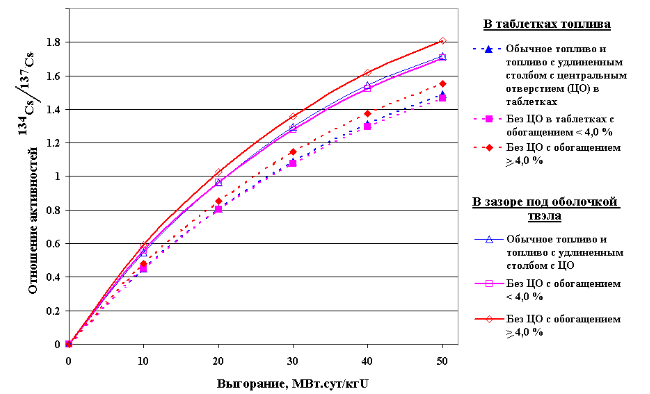
\includegraphics[width=1\linewidth]{pics/ris3} % изображения хранятся в подкаталоге pics
	\caption{Расчетные соотношения активностей радионуклидов $^{134}$Cs и $^{137}$Cs в топливе и в зазоре под оболочкой твэлов в функции выгорания для типичных историй облучения топлива реакторов ВВЭР-1000.~\cite{RD}}
	\label{fig:ris3} % эта метка позволяет ссылаться на рисунок в тексте
\end{figure}

2. Совпадение (с учетом неопределенностей) полученных таким образом
выгораний топлива с выгораниями топлива этих же ТВС по данным
физических расчетов (с учетом неравномерности энерговыделения и
выгорания по высоте и радиусу кассеты) является дополнительным фактом,
подтверждающим наличие негерметичных твэлов в составе контролируемых
ТВС.